\documentclass{ximera}

\title{Vectorcomponenten}
%\author{Daan Lipkens} %uit KUL zomercursus

\begin{document}
\begin{abstract}
    Het beschrijven van vectoren in een assenstelsel, eenheidsvectoren, vectorcomponenten en de norm van een vector.
\end{abstract}
\maketitle

\section{Vectoren in een assenstelsel}

Wanneer we vectoren in een vlak of in de ruimte willen beschrijven, hebben we een assenstelsel nodig. Deze assen kiezen we orthogonaal (loodrecht) met eenzelfde eenheid op iedere as: ze vormen een zogenaamd \textbf{cartesiaans assenstelsel}. Conventioneel worden de assen voor een vlak benoemd met $x$ en $y$. 

Op elke as definiëren we een vector met lengte $1$, die we de \textbf{eenheidsvector} noemen. We stellen deze voor door $\vec{e}_{x}$ en $\vec{e}_{y}$. De indices $x$ en $y$ duiden de richting aan, namelijk volgens de horizontale $x$-as en de verticale $y$-as. Andere notaties van eenheidsvectoren die je vaak zal tegenkomen zijn $\hat{x}$, $\hat{y}$ of $\hat{i}$, $\hat{j}$.

De eenheidsvectoren $\vec{e}_{x}$ en $\vec{e}_{y}$ vormen een basis voor de vectoren in het $x,y$-vlak. Dit betekent dat je elke vector $\vec{a}$ in het $x,y$-vlak op eenduidige wijze kan ontbinden in \textbf{vectorcomponenten} volgens $\vec{e}_{x}$ en $\vec{e}_{y}$:
\[ \vec{a} = \vec{a}_{x} + \vec{a}_{y} = a_{x} \cdot \vec{e}_{x} + a_{y} \cdot \vec{e}_{y} \] 

%---------------------------
% AFBEELDING: Vector ontbinden
\begin{figure}[ht!]
    \captionsetup{width=0.85\textwidth}
    \begin{center}
        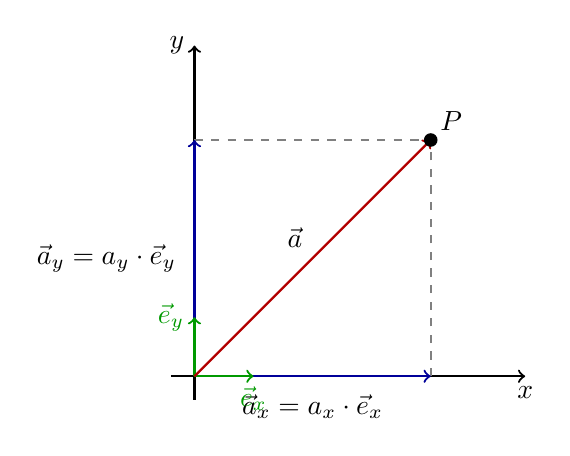
\begin{tikzpicture}[scale=1.5]
            % Assen
            \draw[->, thick] (-0.2, 0) -- (2.8, 0) node[below] {$x$};
            \draw[->, thick] (0, -0.2) -- (0, 2.8) node[left] {$y$};
            
            % Punten
            \coordinate (O) at (0,0);
            \coordinate (P) at (2,2);
            \coordinate (X) at (2,0);
            \coordinate (Y) at (0,2);
            
            % Projectielijnen
            \draw[dashed, gray, thick] (X) -- (P);
            \draw[dashed, gray, thick] (Y) -- (P);
            
            % Vectorcomponenten
            \draw[->, thick, blue!60!black] (O) -- (X) node[midway, below=3pt, text=black] {$\vec{a}_x = a_x \cdot \vec{e}_x$};
            \draw[->, thick, blue!60!black] (O) -- (Y) node[midway, left=3pt, text=black] {$\vec{a}_y = a_y \cdot \vec{e}_y$};
            
            % Eenheidsvectoren
            \draw[->, thick, green!60!black] (O) -- (0.5, 0) node[below] {$\vec{e}_x$};
            \draw[->, thick, green!60!black] (O) -- (0, 0.5) node[left] {$\vec{e}_y$};
            
            % Hoofdvector
            \draw[->, thick, red!70!black] (O) -- (P) node[midway, above left, text=black] {$\vec{a}$};
            
            % Punt aanduiding
            \filldraw[black] (P) circle (1.5pt) node[above right] {$P$};
        \end{tikzpicture}
    \end{center}
    \caption{Vector $\vec{a}$ in een $x,y$-assenstelsel ontbonden in componenten.}
    \label{fig:vectorcomponenten}
\end{figure}
%---------------------------

Aan de hand van de tekening in figuur \ref{fig:vectorcomponenten} definiëren we de volgende termen:
\begin{itemize}
    \item $\vec{a}_{x} = a_{x} \cdot \vec{e}_{x}$ is de \textbf{vectoriële component} van $\vec{a}$ volgens $\vec{e}_{x}$. 
    \item $a_{x}$ noemen we de \textbf{scalaire of algebraïsche component} volgens de $x$-as. 
    \item Analoog is $\vec{a}_{y} = a_{y} \cdot \vec{e}_{y}$ de \textbf{vectoriële component} van $\vec{a}$ volgens $\vec{e}_{y}$. 
    \item $a_{y}$ noemen we de \textbf{scalaire of algebraïsche component} volgens de $y$-as.
\end{itemize}

\begin{example}[title={Vectorcomponenten aflezen op een rooster}]\nl
    \begin{center}
        \captionsetup{width=0.85\textwidth}
        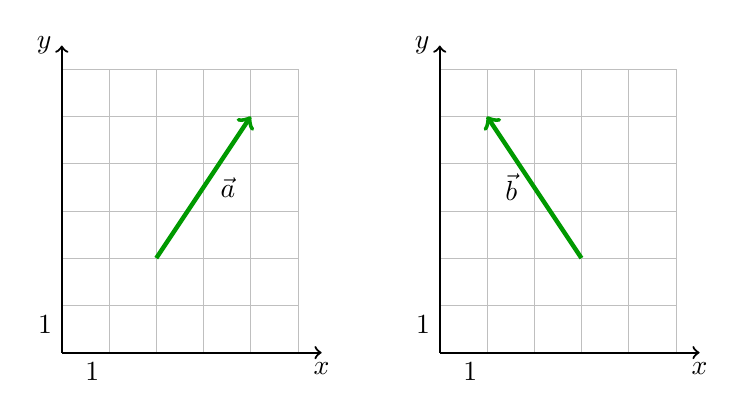
\begin{tikzpicture}[scale=0.6]
            % Rooster 1
            \draw[step=1cm, lightgray, very thin] (0,0) grid (5,6);
            \draw[->, thick] (0,0) -- (5.5,0) node[below] {$x$};
            \draw[->, thick] (0,0) -- (0,6.5) node[left] {$y$};
            \node[below left] at (1,0) {$1$};
            \node[below left] at (0,1) {$1$};
            
            \draw[->, ultra thick, green!60!black] (2,2) -- (4,5) node[midway, right=2pt, text=black] {$\vec{a}$};
            
            % Rooster 2
            \begin{scope}[shift={(8,0)}]
                \draw[step=1cm, lightgray, very thin] (0,0) grid (5,6);
                \draw[->, thick] (0,0) -- (5.5,0) node[below] {$x$};
                \draw[->, thick] (0,0) -- (0,6.5) node[left] {$y$};
                \node[below left] at (1,0) {$1$};
                \node[below left] at (0,1) {$1$};
                
                \draw[->, ultra thick, green!60!black] (3,2) -- (1,5) node[midway, left=2pt, text=black] {$\vec{b}$};
            \end{scope}
        \end{tikzpicture}
        \captionof{figure}{Voorbeelden van het aflezen van scalaire componenten op een rooster.}
        \label{fig:componenten_rooster}
    \end{center}
    
    Op het linkse rooster verplaatst vector $\vec{a}$ zich 2 eenheden naar rechts en 3 eenheden naar boven. De scalaire componenten zijn dus $a_{x} = 2$ en $a_{y} = 3$. Je kan schrijven dat $\vec{a} = 2\cdot \vec{e}_{x} + 3\cdot \vec{e}_{y}$ of korter genoteerd: $\vec{a}=(2,3)$.
    
    Op het rechtse rooster verplaatst vector $\vec{b}$ zich 2 eenheden naar links en 3 eenheden naar boven. De scalaire componenten zijn dus $b_{x} = -2$ en $b_{y} = 3$. Je kan schrijven dat $\vec{b} = -2\cdot \vec{e}_{x} + 3\cdot \vec{e}_{y}$ of korter genoteerd: $\vec{b}=(-2,3)$.
\end{example}

De scalaire componenten zijn reële getallen die zowel positief als negatief kunnen zijn, afhankelijk van de richting en zin van de vector.

%---------------------------
% AFBEELDING: 4 Kwadranten
\begin{figure}[ht!]
    \captionsetup{width=0.85\textwidth}
    \begin{center}
        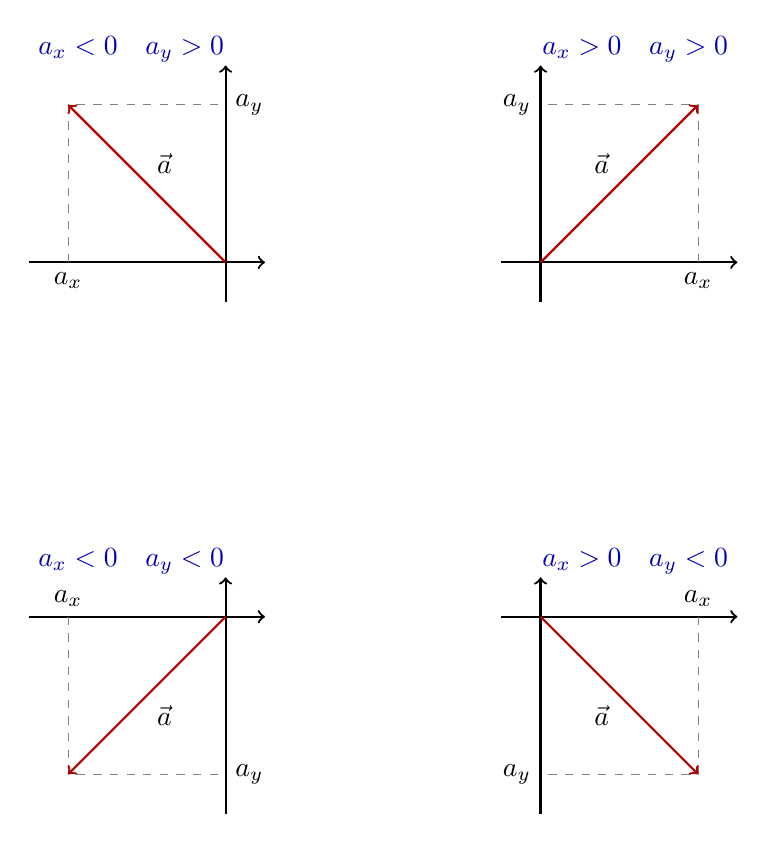
\begin{tikzpicture}[scale=1]
            \tikzset{vec/.style={->, thick, red!70!black}}
            
            % Kwadrant 1 (rechtsboven)
            \begin{scope}[shift={(0,0)}]
                \draw[->, thick] (-0.5,0) -- (2.5,0);
                \draw[->, thick] (0,-0.5) -- (0,2.5);
                \draw[dashed, gray] (2,0) node[below, text=black] {$a_x$} -- (2,2) -- (0,2) node[left, text=black] {$a_y$};
                \draw[vec] (0,0) -- (2,2) node[midway, above left, text=black] {$\vec{a}$};
                \node[blue!70!black] at (1.2, 2.7) {$a_x > 0 \quad a_y > 0$};
            \end{scope}
            
            % Kwadrant 2 (linksboven)
            \begin{scope}[shift={(-4,0)}]
                \draw[->, thick] (-2.5,0) -- (0.5,0);
                \draw[->, thick] (0,-0.5) -- (0,2.5);
                \draw[dashed, gray] (-2,0) node[below, text=black] {$a_x$} -- (-2,2) -- (0,2) node[right, text=black] {$a_y$};
                \draw[vec] (0,0) -- (-2,2) node[midway, above right, text=black] {$\vec{a}$};
                \node[blue!70!black] at (-1.2, 2.7) {$a_x < 0 \quad a_y > 0$};
            \end{scope}

            % Kwadrant 4 (rechtsonder)
            \begin{scope}[shift={(0,-4.5)}]
                \draw[->, thick] (-0.5,0) -- (2.5,0);
                \draw[->, thick] (0,-2.5) -- (0,0.5);
                \draw[dashed, gray] (2,0) node[above, text=black] {$a_x$} -- (2,-2) -- (0,-2) node[left, text=black] {$a_y$};
                \draw[vec] (0,0) -- (2,-2) node[midway, below left, text=black] {$\vec{a}$};
                \node[blue!70!black] at (1.2, 0.7) {$a_x > 0 \quad a_y < 0$};
            \end{scope}

            % Kwadrant 3 (linksonder)
            \begin{scope}[shift={(-4,-4.5)}]
                \draw[->, thick] (-2.5,0) -- (0.5,0);
                \draw[->, thick] (0,-2.5) -- (0,0.5);
                \draw[dashed, gray] (-2,0) node[above, text=black] {$a_x$} -- (-2,-2) -- (0,-2) node[right, text=black] {$a_y$};
                \draw[vec] (0,0) -- (-2,-2) node[midway, below right, text=black] {$\vec{a}$};
                \node[blue!70!black] at (-1.2, 0.7) {$a_x < 0 \quad a_y < 0$};
            \end{scope}
        \end{tikzpicture}
    \end{center}
    \caption{Voorbeelden van vector $\vec{a}$ in verschillende kwadranten.}
    \label{fig:kwadranten}
\end{figure}
%---------------------------


\section{Goniometrie en vectorcomponenten}

In vele situaties is zowel de lengte van de vector als de hoek tussen de vector en één van de assen gekend. In figuur \ref{fig:vector_hoeken} is de hoek $\alpha$ aangeduid tussen de vector $\vec{a}$ en de $x$-as, en de hoek $\alpha'$ tussen de vector en de $y$-as.

%---------------------------
% AFBEELDING: Goniometrie hoeken
\begin{figure}[ht!]
    \captionsetup{width=0.85\textwidth}
    \begin{center}
        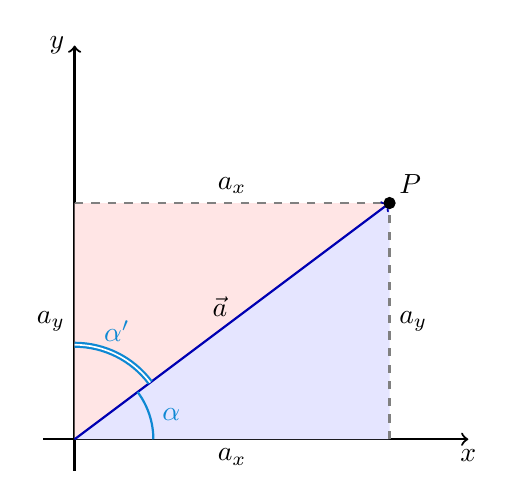
\begin{tikzpicture}[scale=2]
            % Assen
            \draw[->, thick] (-0.2, 0) -- (2.5, 0) node[below] {$x$};
            \draw[->, thick] (0, -0.2) -- (0, 2.5) node[left] {$y$};
            
            % Punten
            \coordinate (O) at (0,0);
            \coordinate (P) at (2,1.5);
            \coordinate (X) at (2,0);
            \coordinate (Y) at (0,1.5);
            
            % Vlakken kleuren
            \fill[blue!10] (X) -- (O) -- (P) -- cycle;
            \fill[red!10] (Y) -- (O) -- (P) -- cycle;
            
            % Projectielijnen
            \draw[dashed, gray, thick] (X) -- (P);
            \draw[dashed, gray, thick] (Y) -- (P);
            
            % Vector
            \draw[->, thick, blue!70!black] (O) -- (P) node[midway, above left=-2pt, text=black] {$\vec{a}$};
            
            % Componenten labels op de randen van de driehoeken
            \node[below] at (1,0) {$a_x$};
            \node[left] at (0,0.75) {$a_y$};
            \node[right] at (2,0.75) {$a_y$};
            \node[above] at (1,1.5) {$a_x$};
            
            % Hoeken
            \draw[thick, cyan!70!blue] (0.5,0) arc (0:36.87:0.5) node[midway, right=1pt] {$\alpha$};
            \draw[thick, cyan!70!blue, double] (0,0.6) arc (90:36.87:0.6) node[midway, above=1pt] {$\alpha'$};
            
            % Punten aanduiden
            \filldraw[black] (P) circle (1pt) node[above right] {$P$};
        \end{tikzpicture}
    \end{center}
    \caption{Vector $\vec{a}$ en de hoeken $\alpha$ en $\alpha'$ met de assen.}
    \label{fig:vector_hoeken}
\end{figure}
%---------------------------

\textbf{Bewijs:} Door de vector $\vec{a}$ te splitsen in zijn componenten, vind je in figuur \ref{fig:vector_hoeken} een blauwe rechthoekige driehoek waarin de hoek $\alpha$ voorkomt. De schuine zijde van deze driehoek heeft lengte $a$, de rechthoekszijden hebben lengte $a_x$ en $a_y$. Door de goniometrische formules voor sinus en cosinus te gebruiken, bekom je:
\begin{align*}
    \cos \alpha &= \frac{a_x}{a} \quad \text{en dus is} \quad a_x = a \cdot \cos \alpha \\
    \sin \alpha &= \frac{a_y}{a} \quad \text{en dus is} \quad a_y = a \cdot \sin \alpha
\end{align*}     

Indien je de hoek $\alpha '$ tussen de vector $\vec{a}$ en de $y$-as zou gebruiken (de rode driehoek), bekom je uiteraard exact dezelfde componenten, maar de gebruikte formules zijn omgewisseld:
\begin{align*}
    \cos \alpha' &= \frac{a_y}{a} \quad \text{en dus is} \quad a_y = a \cdot \cos \alpha' \\
    \sin \alpha' &= \frac{a_x}{a} \quad \text{en dus is} \quad a_x = a \cdot \sin \alpha'
\end{align*} 

\textbf{Omgekeerd:} indien de scalaire componenten van vector $\vec{a}$ gekend zijn, kan men als volgt de hoek $\alpha$ die de vector met de horizontale richting maakt, berekenen:
\[ \alpha = \arctan\left(\frac{|a_{y}|}{|a_{x}|}\right) \] 
    

\section{Lengte of norm}

De lengte of norm van de vector $\vec{a} = a_{x} \cdot \vec{e}_{x} + a_{y} \cdot \vec{e}_{y}$ kan worden berekend via:
\[ a = \| \vec{a} \| = \sqrt{a_{x}^{2} + a_{y}^{2}} \] 
Dit is een rechtstreeks gevolg van de stelling van Pythagoras die geldt in een rechthoekige driehoek.

\begin{theorem}[title={Besluit: Vectorcomponenten en norm}]\nl
    De vector $\vec{a}$ is volledig bepaald als zijn scalaire componenten volgens de assen gekend zijn. We noteren: $\vec{a} = (a_{x}, a_{y})$.
    
    Hieruit volgt dat $\vec{a} = \vec{a}_{x} + \vec{a}_{y} = a_{x} \cdot \vec{e}_{x} + a_{y} \cdot \vec{e}_{y}$. De vector $\vec{a}$ is dus de som van zijn vectoriële componenten.
    
    De lengte of norm van de vector is gelijk aan $a = \| \vec{a} \| = \sqrt{a_{x}^{2} + a_{y}^{2}}$.
\end{theorem}

\begin{remark}[expandable=true,title={Vectoren in drie dimensies}]\nl
    Wil je een vector in de driedimensionale ruimte beschrijven, dan heb je drie assen nodig. Orthogonaal op de $x$- en $y$-as wordt de $z$-as ingevoerd. Een vector $\vec{a}$ kan dan ontbonden worden in drie vectorcomponenten:
    \[ \vec{a} = a_{x} \cdot \vec{e}_{x} + a_{y} \cdot \vec{e}_{y} + a_{z} \cdot \vec{e}_{z} \] 
    
    Dan is:
    \[ \vec{a} = (a_{x}, a_{y}, a_{z}) \] 
    en de norm is: 
    \[ a = \| \vec{a} \| = \sqrt{a_{x}^{2} + a_{y}^{2} + a_{z}^{2}} \] 
\end{remark}
     
\end{document}